%! TEX program = xelatex
\documentclass{article}
\usepackage[UTF8]{ctex}
\usepackage[margin=1in]{geometry}
\usepackage[hidelinks]{hyperref}
\usepackage{amsmath}
\usepackage{lmodern}
\usepackage{footnote}
\usepackage{graphicx}
\usepackage{float}
\usepackage{placeins}
\usepackage{xparse}
\usepackage{listings}
\usepackage{fontspec}
\usepackage{color}
\usepackage[table,xcdraw]{xcolor}
\usepackage{colortbl}
\usepackage{fancyhdr}
\usepackage{comment}
\usepackage{textcomp}
\usepackage{titlesec}
\usepackage{titletoc}
\usepackage{longtable}
\usepackage{enumitem}
\usepackage{booktabs}
\usepackage{float}
\usepackage[sort]{natbib}
\usepackage{subfigure}
\usepackage{multirow}
\usepackage{tabularx}
\usepackage{supertabular}
\usepackage{makecell}
\usepackage{tabu}
\usepackage{longtable}
\renewcommand{\thetable}{\arabic{section}-\arabic{table}}
%\usepackage{hyperref}
\graphicspath{{res/}}

\usepackage{etoolbox}
\BeforeBeginEnvironment{tabular}{\zihao{-5}}

\fancypagestyle{plain}{
	\pagestyle{fancy}      %改变章节首页页眉
}

%\pagestyle{fancy}
%\lhead{\kaishu~课程论文~}
%\rhead{\kaishu~2020 年 11 月 5 日}
\cfoot{\thepage}


\setmonofont[
    Contextuals={Alternate},
    ItalicFont = Fira Code      % to avoid font warning
]{Fira Code}
\definecolor{codegreen}{rgb}{0,0.6,0}
\definecolor{codegray}{rgb}{0.5,0.5,0.5}
\definecolor{codepurple}{rgb}{0.58,0,0.82}
\definecolor{backcolour}{rgb}{0.95,0.95,0.92}

\lstset{
	backgroundcolor=\color{backcolour},   
	commentstyle=\color{codegreen},
	keywordstyle=\color{magenta},
	numberstyle=\tiny\color{codegray},
	stringstyle=\color{codepurple},
	basicstyle=\footnotesize,
	breakatwhitespace=false,         
	breaklines=true,                 
	captionpos=b,                    
	keepspaces=true,                 
	numbers=left,                    
	numbersep=5pt,                  
	showspaces=false,                
	showstringspaces=false,
	showtabs=false, 
	%escapebegin=\begin{CJK*}{GBK}{hei},escapeend=\end{CJK*},                 
	tabsize=2
}

\NewDocumentCommand{\inputCode}{ O{matlab} m }{
	{
		\setmainfont{FiraCode Nerd Font}[
		ItalicFont  = FiraCode Nerd Font
		]
		\lstinputlisting[
		basicstyle=\codeF,
		language=#1,
		tabsize=4,
		showstringspaces=false,
		breaklines=true,
		frame=shadowbox,
		framexleftmargin=10mm,
		rulesepcolor=\color{black},
		basicstyle=\small,
		numbers=left,
		xleftmargin=3em,
		]{#2}
	}
}
\renewcommand{\contentsname}{目录}
\titlecontents{chapter}[0em]{\songti\zihao{-4}}{\thecontentslabel\ }{}
{\hspace{.5em}\titlerule*[4pt]{$\cdot$}\contentspage}
\titlecontents{section}[2em]{\vspace{0.1\baselineskip}\songti\zihao{-4}}{\thecontentslabel\ }{}
{\hspace{.5em}\titlerule*[4pt]{$\cdot$}\contentspage}
\titlecontents{subsection}[4em]{\vspace{0.1\baselineskip}\songti\zihao{-4}}{\thecontentslabel\ }{}
{\hspace{.5em}\titlerule*[4pt]{$\cdot$}\contentspage}


\newcolumntype{Y}{>{\centering\arraybackslash}X}
\newcommand{\upcite}[1]{\textsuperscript{\textsuperscript{\cite{#1}}}}
\title{\LARGE 水果生产运输成本问题的建模}

\begin{document}

	\maketitle
	\tableofcontents
	\thispagestyle{empty}
	\newpage
	\setcounter{page}{1}
	\large


	
	\section{摘要}
	\label{par:zhai_yao_}
	\par 题目中2个问题可以分为最短路径问题和产销平衡问题,而这两种问题都有成熟的解决方法。附件中给出了城市之间的距离数据和水果店所在城市与水果店编号之间的对应关系,对于最短路径问题,我们利用表一的城市之间距离数据建立了城市距离的邻接矩阵,利用Floyd算法进行求解,得到各生产基地与各水果店的最短距离和经过的各城市节点。然后我们利用以上求得的数据对问题1建立产销平衡的整数规划,求得最小成本、各生产基地每天的生产总量、从各生产基地到各水果店每天的供应量以及运输该供应量使用的大车和小车数量。
	
	对于问题2,和问题1相同的步骤,我们对存储天数进行了假设,改造了问题1的模型,求解方法类似,最后我们得到了类似问题1的各变量数据,以及得到了存储天数与平均成本呈现负相关的结论。\\
	\textbf{关键词:}最短路径\quad Floyd算法\quad 产销平衡\quad 整数规划
	\section{问题重述}
	某水果连锁是一家水果运输和销售的公司,公司在某省县级及以上城镇设立连锁店。公司规模目前拥有23家连锁店,以及3个生产基地。
	 
	问题1:目前该公司现有3个生产基地、23家连锁店,生产基地设在16号和63号和120号城镇,为23家连锁店提供水果,2017年连锁店的日销售量见附录2。运输方式有两种:大车可载5吨(少于5吨按5吨计),运输成本为2.25元/车公里;小车可载3吨(少于3吨按3吨计),运输成本为1.5元/车公里。请你为公司设计生产基地的日生产量与日配送方案。
	
	问题2:在日生产总量不变的情况下,如果水果在生产基地最多容许保放5日,水果每天的存储费用为0.05元/公斤。请你为公司重新设计生产(不同生产基地的日产量可能变化)与配送方案,平均每隔几天向连锁店配送一次,可使运输和存储成本最低。
	
	\section{问题分析}
	题目中2个问题具有一定的相似性,可以分为最短路径问题和产销平衡问题分别求解。在求解出问题1的基础上对其进行相应的改造,问题2可以类似地求解。
	
	对于问题1,这是个典型的产销平衡问题,即在需求量固定的情况下求最小的运输成本(问题2为运输成本和储存成本),关键在于得到将水果从各个生产基地运输到销售地所需的大车和小车数量,接着需要得到各生产基地的生产总量和发往各销售地的量。其本质是个整数规划问题。而为了求解此问题,需要各城市间距离矩阵,而附件1给出了城市之间的距离,可以使用一定算法求得最短路径,得到生产基地所在城市与水果店所在城市之间的最短距离。
	
	所以我们按照求解最短路径$\rightarrow $给出路径节点$\rightarrow$ 求解产销平衡问题$\rightarrow $求解问题2的带储存天数产销平衡问题 的顺序给出解决方案。
	\section{符号说明}
\begin{table}[H]
	\centering
	\caption{Parameter values}

		\begin{tabularx}{\textwidth}{llll}
			\toprule[1.5pt]
			符号&解释&符号&解释\\
			\midrule
			$i$&生产地序号&$j$&连锁店序号\\
			$A_i$&第$i$个生产地城市&$B_j$&第$j$个销售城市\\
			$a_i$&第$i$个生产地的生产总量&$b_j$&第$j$个销售城市的需求总量\\
			$x_{ij}$&从$i$地运往$j$地的水果量&$d_{ij}$&$i$地到$j$地的最短距离\\
			$l_{ij}$&从$i$地运往$j$地使用的大车数目&$s_{ij}$&从$i$地运往$j$地使用的小车数目\\
			$y$&问题2中水果保存的天数	&$yy$&问题2中水果真正放置的天数\\
			$a_{ik}$&问题2中第$i$个生产地第$k$天的生产量 & &\\
			\bottomrule[1.5pt]
	\end{tabularx}
\end{table}

\begin{table}[H]
	\centering
	\caption{Parameter values}

		\begin{tabularx}{\textwidth}{lY}
			\toprule[1.5pt]
			符号&解释\\
			\midrule
			$i$&生产地序号\\
			$j$&连锁店序号\\
			$A_i$&第$i$个生产地城市\\
			$B_j$&第$j$个销售城市\\
			$a_i$&第$i$个生产地的生产总量\\
			$b_j$&第$j$个销售城市的需求总量\\
			$x_{ij}$&从$i$地运往$j$地的水果量\\
			$d_{ij}$&$i$地到$j$地的最短距离\\
			$l_{ij}$&从$i$地运往$j$地使用的大车数目\\
			$s_{ij}$&从$i$地运往$j$地使用的小车数目\\
			$y$&问题2中水果保存的天数\\
			$yy$&问题2中水果真正放置的天数\\
			$a_{ik}$&问题2中第$i$个生产地第$k$天的生产量 \\
			\bottomrule[1.5pt]
	\end{tabularx}
\end{table}

% Table generated by Excel2LaTeX from sheet 'Sheet1'
\begin{table}[htbp]
	\centering
	\caption{Add caption}
	\resizebox{\textwidth}{!}{%
	\begin{tabular}{ccccccc}
		\toprule[1.5pt]
		\makecell[c]{一哈哈哈 \\ 哈哈哈} & \makecell[c]{彼此彼此 \\ vcv} & \makecell[c]{股份回购} & \makecell[c]{官方大范 \\ 甘迪} & \makecell[c]{有何吩咐} & \makecell[c]{哈哈哈官方} & \makecell[c]{好好干} \\
		\midrule
		48    & 89    & 5     & 7     & 9     & 11    & 13 \\
		58    & 856   & 5     & 7     & 3250  & 4048  & 4846 \\
		57    & 1623  & 5     & 7     & 85    & 85    & 85 \\
		56    & 2390  & 5     & 7     & 1191  & 1456  & 1720 \\
		55    & 3157  & 5     & 7     & 1229  & 1493  & 1756 \\
		\bottomrule[1.5pt]
	\end{tabular}}%
	\label{tab:addlabel4}%
\end{table}%

	\section{基本假设}
	\begin{enumerate}
		\item 各城市的道路是无向的,它们之间构成无向图;
		\item 从附件2的数据可以看出,每个店的需求量都大于5吨,因此车是沿着最短路径直达的,而不会出现到达一个店卸货后继续前往下一个店的情况;
		\item 保放天数只记录存储在生产基地的天数,发货后水果店无法卖出水果的天数不算作保放天数;
		\item 生产基地每天的生产能力是无限的。
	\end{enumerate}
%	\begin{itemize}
%		\item 各城市的道路是无向的,它们之间构成无向图
%		\item 从附件2的数据可以看出,每个店的需求量都大一5吨,因此车是沿着最短路径直达的,而不会出现到达一个店卸货后继续前往下一个店的情况
%	
%	\end{itemize}
	
	\section{模型建立求解与结果分析}

%\zihao{5}{\heiti 问题一}
	\subsection{最短路径问题模型的求解}
	\subsubsection{模型的建立}
	 该问题本质上是无向图的最短路问题。
	 示意图如下:\\
	 还记得开啥会觉得还是大街上的教科书电竞盛典SD卡算法等级双击打开富士康几乎都是宽度防守打法放得开的生活会打开哈哈哈可视电话很多事恢复对方是否很多事恢复邯郸市考核很多事恢复好地方很多事恢复的话合适的和很多时候速度很好的恢复好的好好读书恢复好的很好的和防守打法的机会水电费很多事复活甲都是很多事和的话的时候觉得好的时候都会给大家发公司就换个环境很好的和速度还是大家好伏见稻荷大社好好读书恢复\\\\
	\begin{figure}[H]
		\centering
		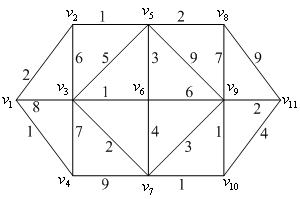
\includegraphics[width=0.55\linewidth]{img/tu.jpg}
		\caption{示意图:无向图的最短路问题}
		\label{fig:shiyitu}
	\end{figure}

    \FloatBarrier
	计算每对顶点之间的最短路径
	计算赋权图中各对顶点之间最短路径,显然可以调用 Dijkstra 算法。这种算法的时间复杂度为$O\left(n^{3}\right)$。第二种解决这一问题的方法是由 Floyd R W 提出的算法,称
	之为Floyd 算法。
	假设图G 权的邻接矩阵$D_0$为:\\
	\begin{center}
	$D_{0}=\left[\begin{array}{cccc}d_{11} & d_{12} & \cdots & d_{1 n} \\ d_{21} & d_{22} & \cdots & d_{2 n} \\ \vdots & \vdots & \cdots & \vdots \\ d_{n 1} & d_{n 2} & \cdots & d_{n n}\end{array}\right]$
	\end{center}
    来存放各边长度,其中:
	$d_{i i}=0 \quad i=1,2, \cdots, n ;$\\
	$d_{i j}=\infty \quad i, j$ 之间没有边,在程序中以各边都不可能达到的充分大的数代替; \\
	$d_{i j}=w_{i j} \quad w_{i j}$ 是 $i, j$ 之间边的长度, $i, j=1,2, \cdots, n$ 。 对于无向图, $A_{0}$ 是对称矩阵,
	 $d_{i j}=d_{j i} $ 。\\
	 Floyd 算法的基本思想是:递推产生一个矩阵序列 $D_{0}, D_{1}, \cdots, D_{k}, \cdots, D_{n},$ 其中$D_{k}(i, j)$ 表示从顶点 $v_{i}$ 到顶点 $v_{j}$ 的路径上所经过的顶点序号不大于 $k$ 的最短路径长度。\\
	 计算时用迭代公式:
	 $$
	 D_{k}(i, j)=\min \left(D_{k-1}(i, j), D_{k-1}(i, k)+D_{k-1}(k, j)\right)
	 $$
	 $k$ 是迭代次数, $i, j, k=1,2, \cdots, n $。
	 最后,当 $k=n$ 时, $A_{n}$ 即是各顶点之间的最短通路值。
	 
	 \subsubsection{模型求解}
	 
	 对附件2的数据进行预处理,我们发现同一城市可能有多个水果店,城市编号和水果店数量的关系如如图\ref{fig:dianshu}所示:
	 \begin{figure}[H]
	 	\centering
	 	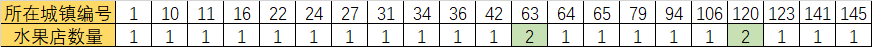
\includegraphics[width=1.0\linewidth]{img/dianshu.png}
	 	\caption{每个城市水果店的数目}
	 	\label{fig:dianshu}
	 \end{figure}
	 
	 可以看到,第63号和第120号城市有2个水果店,为此,我们对在同一城市的水果店的需求量进行了合并,从而有利于后面问题的简化和求解。接着,我们按照水果店所在城市的编号大小进行了重新排序,得到21个需求城市的需求量与编号的对应关系如图\ref{fig:xiaoliang}所示:
	 
	 \begin{figure}[H]
	 	\centering
	 	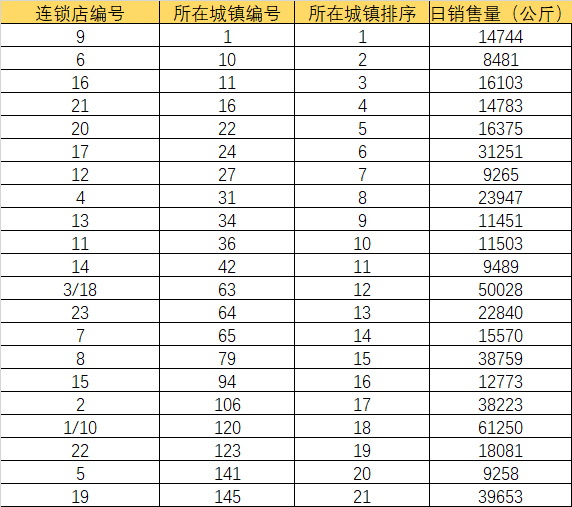
\includegraphics[width=0.8\linewidth]{img/xiaoliang.png}
	 	\caption{21个需求城市的需求量与编号的对应关系}
	 	\label{fig:xiaoliang}
	 \end{figure}
	 
	 有3个生产地城市,21个需求地城市,对附件1中给出城市间距离,我们使用matlab进行了excel数据的读取,建立邻接矩阵,使用Floyd算法求解,得到各城市之间最短距离,然后提取的所需要的各生产基地所在城市到水果店所在城市的最短距离和经过的中间节点。\ref{fig:jvli}所示:
	 
	 \begin{figure}[htpb]
	 	\centering
	 	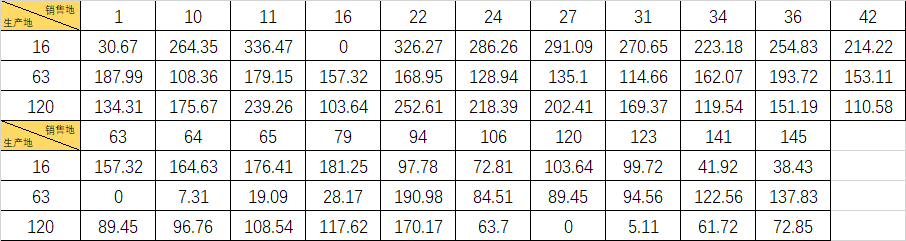
\includegraphics[width=1.0\linewidth]{img/jvli.png}
	 	\caption{各生产地城市与需求地城市的最短距离矩阵}
	 	\label{fig:jvli}
	 \end{figure}
      两两之间经过的节点城市编号列表如图\ref{fig:node}所示(见下页),第1列为起始城市也即生产基地所在城市,每行为各路径的节点,每行末尾数为终止城市,也即销售地城市。
     \begin{figure}[htpb]
     	\centering
     	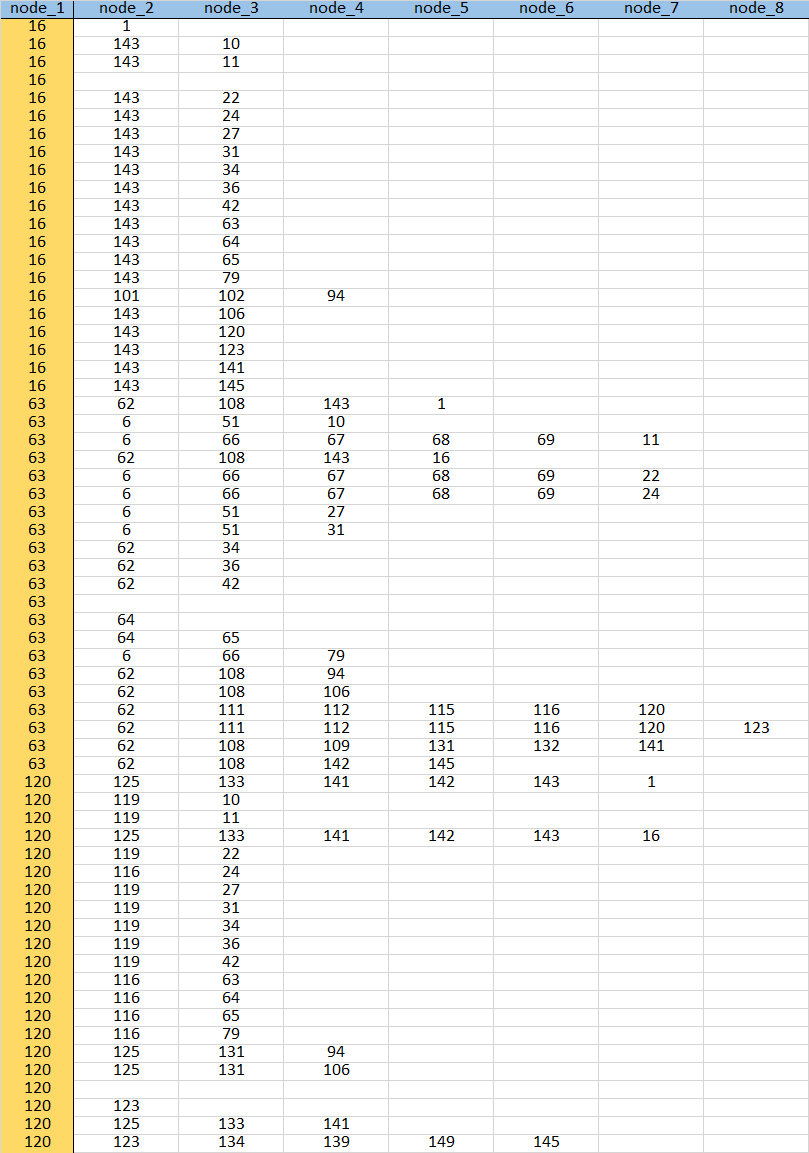
\includegraphics[width=0.95\linewidth]{img/node.png}
     	\caption{两两之间经过的节点城市编号列表}
     	\label{fig:node}
     \end{figure}
	 
	\subsection{产销平衡问题模型的求解}
	\subsubsection{模型的建立}
	运输方式有两种:大车可载5吨(少于5吨按5吨计),运输成本为2.25元/车公里;小车可载3吨(少于3吨按3吨计),运输成本为1.5元/车公里。在满足生产量等于销售量的前提下,使得运输成本尽可能小。可得目标函数为:\\
	\\
	$\min =\sum_{i=1}^{m} \sum_{j=1}^{n}\left(2.25 l_{i j}+1.5 s_{i j}\right) \cdot d_{i j}$\\
	\\
	约束条件如下:
	\begin{itemize}
	    \item 每个产地发往销地的总和等于该产地的生产量;
	    \item 各生产基地发往一个销地的总和等于该销地的需求量;
	    \item 从某产地发往某销地的水果量应该大于0,且等于大车和小车的运输量的和;
	    \item 大车数量和小车数量应该是整数;
	\end{itemize}
	因此,建立如下整数规划模型:\\
	
	$$
	\begin{array}{lr}
		\min =\sum_{i=1}^{m} \sum_{j=1}^{n}\left(2.25 l_{i j}+1.5 s_{i j}\right) \cdot d_{i j} \\
		\\
		\text { s.t. }\quad\left\{\begin{array}{lr}
			\sum_{j=1}^{n} x_{i j}=a_{i} \\
			\sum_{i=1}^{m} x_{i j}=b_{j} \\
			x_{i j} \geq 0 \\
			x_{i j}\leq 5000 l_{i j}+3000 s_{i j}\\
			l_{i j}, s_{i j}  \mbox{为整数}\\
			i=1,2, \ldots m \quad j=1,2, \ldots n \\
			m=3, n=21
			
		\end{array}\right.
	\end{array}
	$$
	\subsubsection{模型的求解}
	对模型进行分析,发现该问题变量较多,不适合用matlab求解,因此我们使用了lingo软件进行计算.
	我们得到目标值为12907.07元。即最低成本为12907.07元,在最优情况下各变量的值如下:\\
	从$i\rightarrow j$的发货量$x_{i j}$的值如图\ref{fig:Xij}所示\\
	从$i\rightarrow j$的大车数目$l_{i j}$的值如图\ref{fig:lij}所示\\
	从$i\rightarrow j$的小车数目$s_{i j}$的值如图\ref{fig:sij}所示\\
	\begin{figure}[H]%htpb
		\centering
		\includegraphics[width=1.0\linewidth]{img/Xij.png}
		\caption{从第$i$个生产地到第$j$销售地的发货量矩阵}
		\label{fig:Xij}
	\end{figure}
	
	\begin{figure}[H]
		\centering
		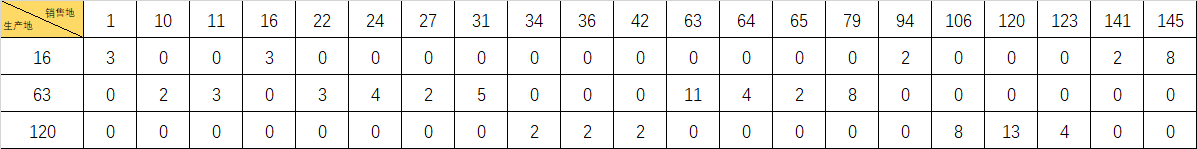
\includegraphics[width=1.0\linewidth]{img/lij.png}
		\caption{从第$i$个生产地到第$j$销售地的所用的大车数量矩阵}
		\label{fig:lij}
	\end{figure}
	
	\begin{figure}[H]
		\centering
		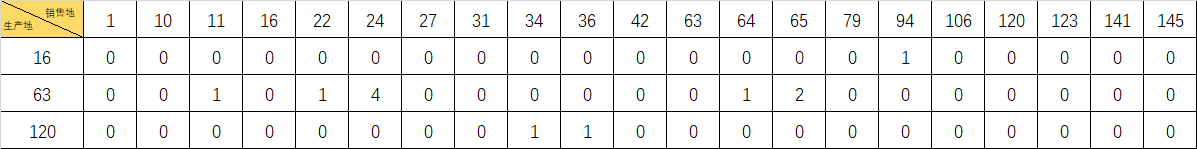
\includegraphics[width=1.0\linewidth]{img/sij.png}
		\caption{从第$i$个生产地到第$j$销售地的所用的小车数量矩阵}
		\label{fig:sij}
	\end{figure}

    得到的结果是城市与城市之间的发货量,转换为生产基地与各水果店的发货量时,对于一个城市有多个水果店的情况,只需要将发往该城市的货量按照各水果店的需求量进行相应的分配即可,对于一个城市只有一个水果店的情况,则直接发货。
   \\
   \\
	%\zihao{4}{\heiti 问题二}
	\subsection{问题二模型的求解}
	\subsubsection{模型的建立}
	同问题1,根据题意,我们假设水果在生产基地存储$y$天\\
	$a_{ik}$为第$i$个生产地出货日前第$k$天的生产量, $yy=y+1$ 表示实际放置的天数(保放天数加上当天1天)
	成本应为(运输成本+保放成本)/(保放天数+1),所以建立如下整数规划:
	$$
	\begin{array}{lr}
	\min =\frac{\sum_{i=1}^{m} \sum_{j=1}^{n}\left(2.25 l_{i j}+1.5 s_{i j}\right) \cdot d_{i j} +0.05 \sum_{i=1}^{m} \sum_{k=1}^{y} a_{i k}}{yy}\\
	\\
	\text { s.t. }\quad\left\{\begin{array}{lr}
	    \sum_{j=1}^{n} x_{i j}=\sum_{k=1}^{yy} a_{i k} \\
	    \sum_{i=1}^{m} x_{i j}=b_{j}\cdot (y+1) \\
		x_{i j} > 0 \\
		x_{i j}\leq 5000 l_{i j}+3000 s_{i j}\\
		l_{i j}, s_{i j}  \mbox{为整数}\\
		yy=y+1\\
		i=1,2, \ldots m \quad j=1,2, \ldots n\quad k=1,2, \ldots y\\
		m=3, n=21\\
		y\leq 5
	
       \end{array}\right.
   \end{array}
    $$
	\subsubsection{模型的求解}
	使用Lingo程序,设置y的值分别为1,2,3,4,5,得到目标函数值如图\ref{fig:chengben}所示:
	\begin{figure}[H]
		\centering
		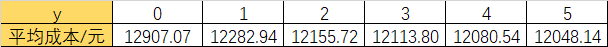
\includegraphics[width=1.0\linewidth]{img/chengben.png}
		\caption{从第$i$个生产地到第$j$销售地的所用的小车数量矩阵}
		\label{fig:chengben}
	\end{figure}
    保放天数$y$与平均成本的关系如图\ref{fig:qvxian}所示
	\begin{figure}[H]
		\centering
		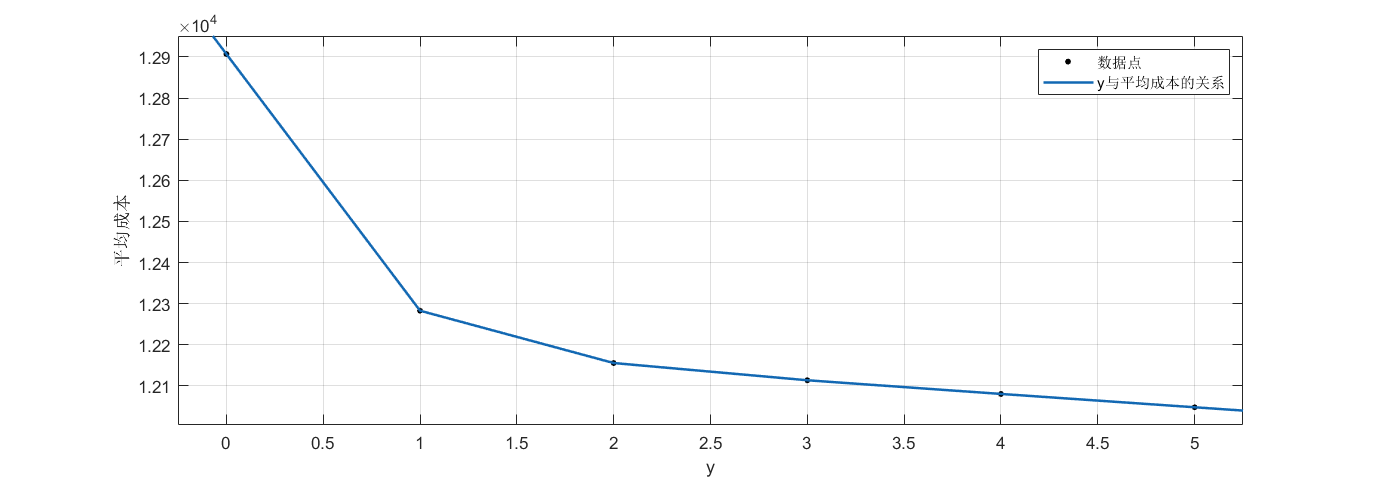
\includegraphics[width=1.0\linewidth]{img/qvxian.png}
		\caption{从第$i$个生产地到第$j$销售地的所用的小车数量矩阵}
		\label{fig:qvxian}
	\end{figure}
    \par 由曲线可知,平均成本随着y的增大而减小,因此保放5天成本最低。\\
    y=1,2,3,4,5时个生产基地每天的生产量如图\ref{fig:duotu}所示
    \begin{figure}[htbp]
    	\centering
    	\subfigure[$y=1$]{
    		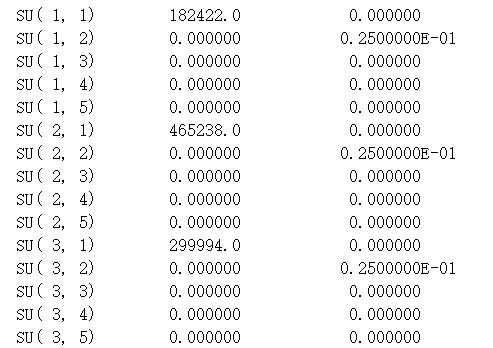
\includegraphics[width=0.45\linewidth]{img/y=1.png}
    		%\caption{fig1}
    	}
    	\quad
    	\subfigure[$y=2$]{
    		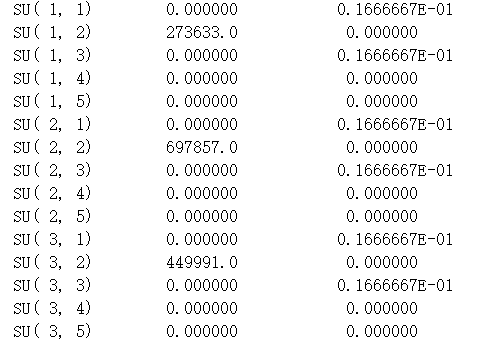
\includegraphics[width=0.45\linewidth]{img/y=2.png}
    	}
    	\quad
    	\subfigure[$y=3$]{
    		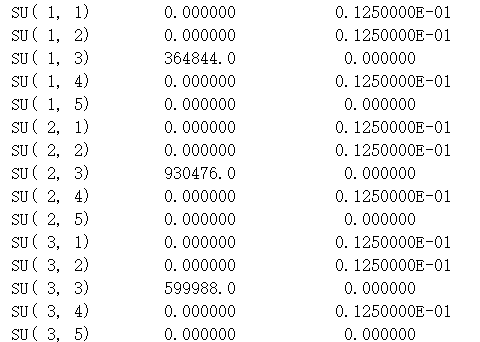
\includegraphics[width=0.45\linewidth]{img/y=3.png}
    	}
    	\quad
    	\subfigure[$y=4$]{
    		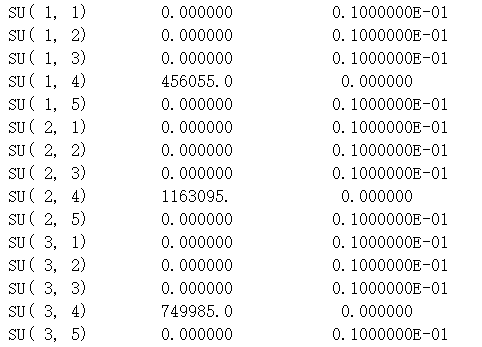
\includegraphics[width=0.45\linewidth]{img/y=4.png}
	    	}
	    \quad
	    \subfigure[$y=5$]{
	    	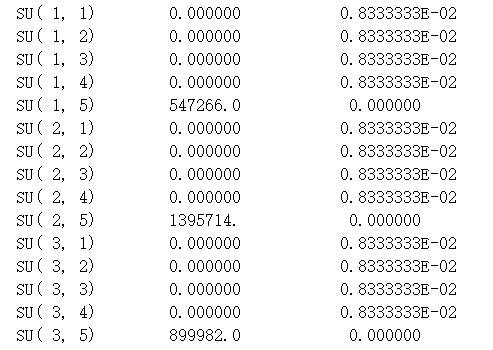
\includegraphics[width=0.45\linewidth]{img/y=5.png}
	    }
    	\caption{ y=1,2,3,4,5时个生产基地每天的生产量}
    	\label{fig:duotu}
    \end{figure}
    
    分析lingo程序运行结果,如图\ref{fig:duotu}所示,可以得知:无论y的值是多少,水果都是当天生产当天发出,也就是说没有保放的水果。\\
    下面是保放5天时的各变量数据:\\
    3处生产基地该天的生产量如图\ref{fig:shengchanliang}所示\\
	从$i\rightarrow j$的发货量$x_{i j}$的值如图\ref{fig:xij2}所示\\
	从$i\rightarrow j$的大车数目$l_{i j}$的值如图\ref{fig:lij2}所示\\
	从$i\rightarrow j$的小车数目$s_{i j}$的值如图\ref{fig:sij2}所示\\
	\begin{figure}[H]%htpb
		\centering
		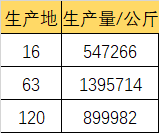
\includegraphics[width=0.25\linewidth]{img/shengchanliang.png}
		\caption{3处生产基地该天的生产量}
		\label{fig:shengchanliang}
	\end{figure}
	\begin{figure}[H]%htpb
		\centering
		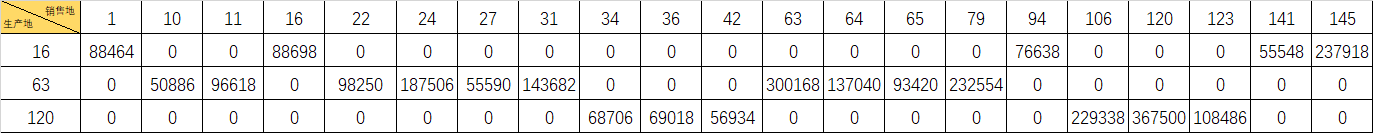
\includegraphics[width=1.0\linewidth]{img/xij2.png}
		\caption{y=5时从第$i$个生产地到第$j$个销售地的发货量矩阵}
		\label{fig:xij2}
	\end{figure}
	
	\begin{figure}[H]
		\centering
		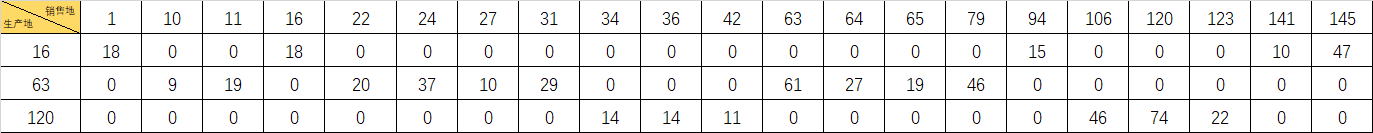
\includegraphics[width=1.0\linewidth]{img/lij2.png}
		\caption{y=5时从第$i$个生产地到第$j$个销售地的所用的大车数量矩阵}
		\label{fig:lij2}
	\end{figure}
	
	\begin{figure}[H]
		\centering
		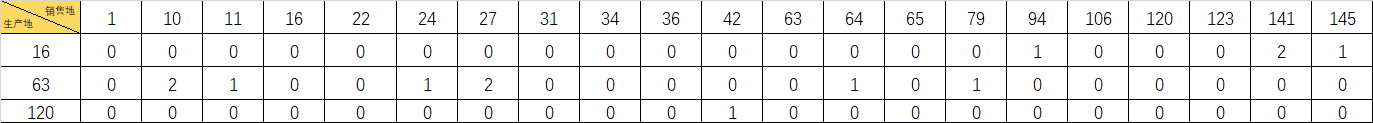
\includegraphics[width=1.0\linewidth]{img/sij2.png}
		\caption{y=5时从第$i$个生产地到第$j$个销售地的所用的小车数量矩阵}
		\label{fig:sij2}
	\end{figure}
	
	
	\section{结果分析}
	对问题1进行灵敏度分析:\\
	问题1 $l_{i j}$和$s_{i j}$的Reduced Cost值如图\ref{fig:lingmingdu}所示:\\
	\begin{figure}[htbp]
		\centering
		\subfigure[$l_{i j}$的Reduced Cost值]{
			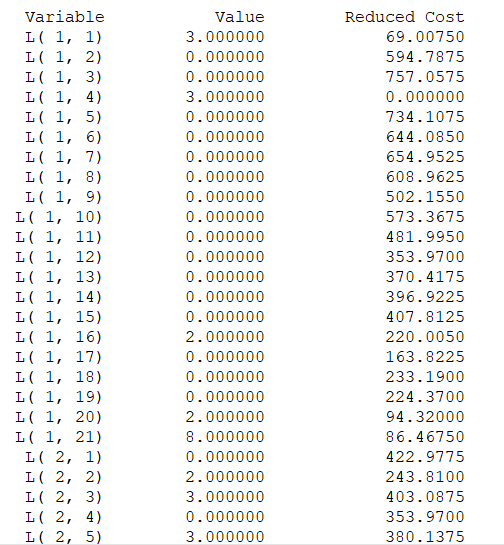
\includegraphics[width=0.47\linewidth]{img/lingmingdu.png}
			%\caption{fig1}
		}
		\quad
		\subfigure[$s_{i j}$的Reduced Cost值]{
			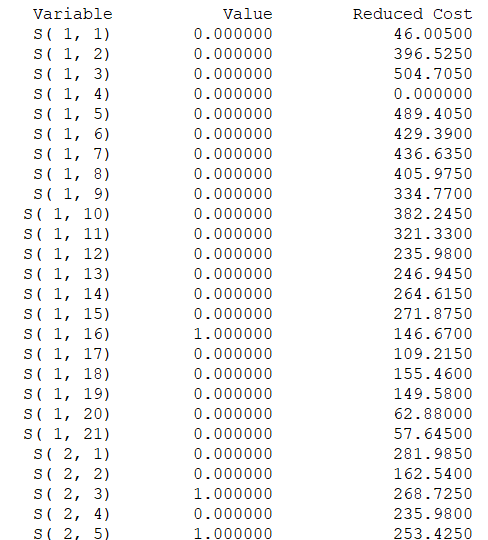
\includegraphics[width=0.47\linewidth]{img/lingmingdu2.png}
		}
		\caption{ $s_{i j}$和$l_{i j}$的Reduced Cost值}
		\label{fig:lingmingdu}
	\end{figure}

    可以看到$l_{i j}$(大车)的Reduced Cost值大多在300-700,$s_{i j}$(小车)的Reduced Cost值大多在100-400,说明大车的数量变化对结果的影响更大一些,这与实际情况也是相符的。
	
	
	\section{模型优缺点及改进方向}
	\begin{itemize}
		\item \textbf{优点:}本文模型较为全面地分析了运输成本的优化问题,建立了从求解最短路径$\rightarrow $给出路径节点$\rightarrow$ 求解产销平衡问题$\rightarrow $求解问题2的带储存天数产销平衡问题等一系列问题的解决方案, 
		\item \textbf{缺点:}在算法上还有很多不足,比如求解问题2时,Lingo程序基础不牢,导致求和上限为变量的程序不知道如何编写,导致y值只能一个一个地试。
		\item \textbf{改进方向:}我们假设生产基地的每天生产能力为无限,实际上其不可能为无限。如果能够得到生产能力上限的数据,可以对模型进行改进与优化;另外,水果的保存天数应该等于在生产基地和销售地保存天数的总和,如果有水果店的销售时间数据,也可对模型作进一步的改进。
	\end{itemize}
	
	


    \section{附录}
	\appendix
	\section{求最短路径的matlab程序}
	%\inputCode[matlab]{mindistance.m}
%	\lstinputlisting[language=matlab]{mindistance.m}
%	\lstinputlisting[language=python]{main.py}
	\begin{lstlisting}[language=matlab]
	clear;warning('off');
	n=154; d=zeros(n);
	x=xlsread('1.xlsx');
	start=floor(x(:,1));ending=floor(x(:,2));dij=x(:,3);
	for i=1:length(start)
	    d(start(i),ending(i))=dij(i);
	end
	d=d+d'; 
	d(d==0)=inf; %把所有零元素替换成无穷
	d([1:n+1:n^2])=0; %对角线元素替换成零,Matlab中数据是逐列存储的
	[d_all,path]=myfloyd(d);
	startcity=[16,63,120];
	endcity=[1,10,11,16,22,24,27,31,34,36,42,63,64,65,79,94,106,120,123,141,145];
	d_simp=d_all(startcity,endcity);
	xlswrite('distance.xlsx',d_simp);
	% figure(1);
	mypath=cell(length(startcity)*length(endcity),1);
	for i=1:length(startcity)
	    for j=1:length(endcity)
	        sb=startcity(i);db=endcity(j);
	        mypath((i-1)*length(endcity)+j,1)={findpath(path,sb,db)};
	    end
	end
	m=cell2table(mypath);
	writetable(m,'node.xlsx')
	
	function [dist,mypath]=myfloyd(a)
	% 输入:a—邻接矩阵,元素(aij)是顶点i到j之间的直达距离,可以是有向的
	% sb—起点的标号;db—终点的标号
	% 输出:dist—最短路的距离;% mypath—最短路的路径
	n=size(a,1); path=zeros(n);
	for k=1:n
	    for i=1:n
	        for j=1:n
	           if a(i,j)>a(i,k)+a(k,j)
	               a(i,j)=a(i,k)+a(k,j);
	               path(i,j)=k;
	           end
	        end
	    end
	end
	dist=a;
	mypath=path;
	end
	
	function mypath=findpath(path,sb,db)
	parent=path(sb,:); %从起点sb到终点db的最短路上各顶点的前驱顶点
	parent(parent==0)=sb; %path中的分量为0,表示该顶点的前驱是起点
	mypath=db; t=db;
	while t~=sb
	    p=parent(t); mypath=[p,mypath];
	    t=p;
	end
	end
	\end{lstlisting}
	\section{求解问题一的lingo程序}
	\label{sec:corn_field_poj_3254_suan_fa_yuan_dai_ma_}
	\begin{lstlisting}[language=lingo]
	sets:
	supplys/1..3/: A;
	demands/1..21/: B;
	links(supplys, demands): x, d, l, s;
	endsets
	
	data:
	B = 14744 8481 16103 14783 16375 31251 9265 23947 11451 11503 9489 50028 22840 15570 38759 12773 38223 61250 18081 9258 39653;	
	d = 30.67 264.35 336.47 0 326.27 286.26 291.09 270.65 223.18 254.83 214.22 157.32 164.63 176.41 181.25 97.78 72.81 103.64 99.72 41.92 38.43 
	187.99 108.36 179.15 157.32 168.95 128.94 135.1 114.66 162.07 193.72 153.11 0 7.31 19.09 28.17 190.98 84.51 89.45 94.56 122.56 137.83 
	134.31 175.67 239.26 103.64 252.61 218.39 202.41 169.37 119.54 151.19 110.58 89.45 96.76 108.54 117.62 170.17 63.7 0 5.11 61.72 72.85;
	@ole(output.xls,'x') = x;!Run Lingo as an administrator and open this excel file;
	@ole(output.xls,'l') = l;
	@ole(output.xls,'s') = s;
	@ole(output.xls,'a') = a;
	@ole(output.xls,'b') = b;
	@ole(output.xls,'d') = d;
	enddata
	
	min = @sum(links(i,j): (2.25*l(i,j)+1.5*s(i,j)) * d(i,j));
	@for(supplys(i): @sum(demands(j): x(i,j)) = A(i));
	@for(demands(j): @sum(supplys(i): x(i,j)) = B(j));
	@for(links(i,j): @gin(l(i,j)));
	@for(links(i,j): @gin(s(i,j)));
	@for(links(i,j): x(i,j)<=5000*l(i,j)+3000*s(i,j));
	end
	\end{lstlisting}
	\section{求解问题二的lingo程序}
	\begin{lstlisting}[language=lingo]
	sets:
	supplysplace/1..3/: A;
	demands/1..21/: B;
	savedate/1..5/;
	supplys(supplysplace,savedate):su;
	links(supplysplace, demands): x, d, l, s;
	endsets
	
	data:
	B = 14744 8481 16103 14783 16375 31251 9265 23947 11451 11503 9489 50028 22840 15570 38759 12773 38223 61250 18081 9258 39653;	
	d = 30.67 264.35 336.47 0 326.27 286.26 291.09 270.65 223.18 254.83 214.22 157.32 164.63 176.41 181.25 97.78 72.81 103.64 99.72 41.92 38.43 
	187.99 108.36 179.15 157.32 168.95 128.94 135.1 114.66 162.07 193.72 153.11 0 7.31 19.09 28.17 190.98 84.51 89.45 94.56 122.56 137.83 
	134.31 175.67 239.26 103.64 252.61 218.39 202.41 169.37 119.54 151.19 110.58 89.45 96.76 108.54 117.62 170.17 63.7 0 5.11 61.72 72.85;
	@ole(out2.xls,'su') = su;
	@ole(out2.xls,'x') = x;!Run Lingo as an administrator;
	@ole(out2.xls,'l') = l;
	@ole(out2.xls,'s') = s;
	enddata
	min = cost/yy;
	
	cost = @sum(links(i,j): (2.25*l(i,j)+1.5*s(i,j)) * d(i,j))+0.05*@sum(supplysplace(i):A(i)-su(i,y));
	@for(supplysplace(i):A(i)=@sum(supplys(i,k)|k#le#yy:su(i,k)));
	@for(supplysplace(i): @sum(demands(j): x(i,j)) = A(i));
	@for(demands(j): @sum(supplysplace(i): x(i,j)) = B(j)*yy);
	yy=y+1;
	y=5;!y=1,2,3,4,5;
	@gin(y);
	@for(links(i,j): @gin(l(i,j)));
	@for(links(i,j): @gin(s(i,j)));
	@for(links(i,j): x(i,j)<=5000*l(i,j)+3000*s(i,j));
	end
	\end{lstlisting}
	\addcontentsline{toc}{section}{参考文献}
%	\begin{thebibliography}{}
%%		\bibitem{liu} 刘海洋. \LaTeX 入门 [M]. 北京: 电子工业出版社, 2013.
%%		\bibitem{hu}  胡伟. \LaTeX 2e完全学习手册(第二版). 北京: 清华大学出版社, 2013.
%	\end{thebibliography}
	\bibliographystyle{unsrt}
	\bibliography{ref.bib}
%	\begingroup
%	\renewcommand{\section}[2]{}%
%	\nocite{*}
%	\bibliographystyle{unsrt}
%	\bibliography{ref.bib}
%	\endgroup
		
\end{document}